% Customizable fields and text areas start with % >> below.
% Lines starting with the comment character (%) are normally removed before release outside the collaboration, but not those comments ending lines

% svn info. These are modified by svn at checkout time.
% The last version of these macros found before the maketitle will be the one on the front page,
% so only the main file is tracked.
% Do not edit by hand!
\RCS$Revision: 401814 $
\RCS$HeadURL: svn+ssh://svn.cern.ch/reps/tdr2/notes/DN-17-002/trunk/DN-17-002.tex $
\RCS$Id: DN-17-002.tex 401814 2017-05-01 14:27:52Z ntran $
%%%%%%%%%%%%% local definitions %%%%%%%%%%%%%%%%%%%%%
% This allows for switching between one column and two column (cms@external) layouts
% The widths should  be modified for your particular figures. You'll need additional copies if you have more than one standard figure size.
\newlength\cmsFigWidth
\ifthenelse{\boolean{cms@external}}{\setlength\cmsFigWidth{0.85\columnwidth}}{\setlength\cmsFigWidth{0.4\textwidth}}
\ifthenelse{\boolean{cms@external}}{\providecommand{\cmsLeft}{top\xspace}}{\providecommand{\cmsLeft}{left\xspace}}
\ifthenelse{\boolean{cms@external}}{\providecommand{\cmsRight}{bottom\xspace}}{\providecommand{\cmsRight}{right\xspace}}
%%%%%%%%%%%%%%%  Title page %%%%%%%%%%%%%%%%%%%%%%%%
\cmsNoteHeader{DN-17-002} % This is over-written in the CMS environment: useful as preprint no. for export versions
% >> Title: please make sure that the non-TeX equivalent is in PDFTitle below
\title{Fast Particle Flow and PUPPI algorithms for the Phase-2 L1 Trigger at CMS}

% >> Authors
%Author is always "The CMS Collaboration" for PAS and papers, so author, etc, below will be ignored in those cases
%For multiple affiliations, create an address entry for the combination
%To mark authors as primary, use the \author* form
\address[cern]{CERN}
\address[fnal]{Fermilab}
\address[nw]{Northwestern University}

\author[cern]{Phil Harris}
\author[fnal]{Benjamin Jonah Kreis}
\author[cern]{Giovanni Petrucciani}
\author[nw]{Stanislava Sevova}
\author[nw]{Kevin Sung}
\author[fnal]{Nhan Tran}

% >> Date
% The date is in yyyy/mm/dd format. Today has been
% redefined to match, but if the date needs to be fixed, please write it in this fashion.
% For papers and PAS, \today is taken as the date the head file (this one) was last modified according to svn: see the RCS Id string above.
% For the final version it is best to "touch" the head file to make sure it has the latest date.
\date{\today}

% >> Abstract
% Abstract processing:
% 1. **DO NOT use \include or \input** to include the abstract: our abstract extractor will not search through other files than this one.
% 2. **DO NOT use %**                  to comment out sections of the abstract: the extractor will still grab those lines (and they won't be comments any longer!).
% 3. For PASs: **DO NOT use tex macros**         in the abstract: CDS MathJax processor used on the abstract doesn't understand them _and_ will only look within $$. The abstracts for papers are hand formatted so macros are okay.
\abstract{
This document describes the development and validation of a fast particle flow-like algorithm to be used in CMS L1 trigger applications.
The particle flow reconstruction algorithm has been successfully demonstrated at CMS.
In high pileup scenarios, the pileup per particle identification (PUPPI) algorithm, used in conjunction with particle flow, has been demonstrated to greatly mitigate the physics performance degradation from pileup.  
In this dectector performance note, we adapt these algorithms for use in a "level-1"
hardware trigger proposed for CMS during the HL-LHC runs.
We develop a simplified fast algorithm and study its physics performance with respect to other trigger algorithms and the offline reconstruction.  
We also study the feasilibity of implementing this algorithm in firmware and benchmark its performance.
}

% >> PDF Metadata
% Do not comment out the following hypersetup lines (metadata). They will disappear in NODRAFT mode and are needed by CDS.
% Also: make sure that the values of the metadata items are sensible and are in plain text:
% (1) no TeX! -- for \sqrt{s} use sqrt(s) -- this will show with extra quote marks in the draft version but is okay).
% (2) no %.
% (3) No curly braces {}.
\hypersetup{%
pdfauthor={Phil Harris, Ben Kreis, Giovanni Petrucciani, Stanislava Sevova, Nhan Tran},%
pdftitle={Performance of Particle Flow and Fast PUPPI algorithm for the Phase 2 L1 Trigger at CMS},%
pdfsubject={CMS},%
pdfkeywords={CMS, physics, software, computing}}

\maketitle %maketitle comes after all the front information has been supplied
% >> Text
%%%%%%%%%%%%%%%%%%%%%%%%%%%%%%%%  Begin text %%%%%%%%%%%%%%%%%%%%%%%%%%%%%
%% **DO NOT REMOVE THE BIBLIOGRAPHY** which is located before the appendix.
%% You can take the text between here and the bibiliography as an example which you should replace with the actual text of your document.
%% If you include other TeX files, be sure to use "\input{filename}" rather than "\input filename".
%% The latter works for you, but our parser looks for the braces and will break when uploading the document.
%%%%%%%%%%%%%%%
\tableofcontents

\clearpage
\section{Introduction}
\label{sec:intro}
The physics program of CMS has achieved incredible results in its first 2 runs including the discovery of the Higgs boson.
The Higgs discovery completes the standard model (SM) of particle physics.  
Despite this incredible achievement, many mysteries beyond the (SM) remain including understanding the hierarchy problem,
the nature of dark matter, and the origin of the matter-antimatter asymmetry in the universe.  

Therefore, the CMS program continues to study the SM in great detail and probe for signs of beyond the SM physics.  
For the continued success of CMS physics program, CMS plans accumulate an unprecedented amount of data, approximately $3~ab^\text{-1}$, to be delivered by the (high luminosity) HL-LHC.  
This dataset will be approximately 100 times larger than our current LHC dataset.  
Although we will accumulate an unprecendented dataset, we will have to deal with increasingly complex enviroments characterized by
extreme levels of pileup.  
Pileup is defined as p-p interactions, produced in addition to the interaction of interest.
They serve to add noise to the detection of particular physics processes and degrade the performance and sensitivity of CMS.
During the HL-LHC runs, there are expected to be approximately 140-200 pileup interactions per proton bunch crossing. 
So while we will have an unprecedented amount of data, we will need to maintain the current physics performance of the CMS detector in order to maximize the HL-LHC run.

In particular, one primary issue related to the additional pileup is the increased trigger rates.  
The purpose of CMS trigger system is to determine and save the most interesting physics events.
Without an efficient trigger system we would not save the right events to permanent storage and would thus lose important physics. 
The collision rate at the (HL-)LHC is 40~MHz.  
The trigger system, during the HL-LHC, will be required to reduce that rate to a more manageable rate of $\sim5~$KHz~\cite{Contardo:2020886}.  
This data reduction occurs through a 2-layer system: in level-1 (L1), hardware and fast electronics are used to reduce the rate to approximately 700~KHz; and in the second layer, the high level trigger (HLT), the rate is reduced down to approxiately 5~KHz.  
We focus in this document on the design and implementation of a L1 hardware trigger.  
External constraints and the size of detector buffers constrain the time of the L1 decision to be approximately $12.5~\mu s$.  
The L1 trigger system includes information from the calorimeters and muon systems, and new for the HL-LHC, it will also include tracker information.  
The system is illustrated in Fig.~\ref{fig:overview}.
In this document we focus on the design and performance of the "correlator" system, denoted in Fig.~\ref{fig:overview}.
With the new tracking information avaialable in the L1 trigger for the HL-LHC, the L1 trigger algorithms can be completely 
redesigned and the perforamnce can be greatly improved.

\begin{figure}[htb]
\centering
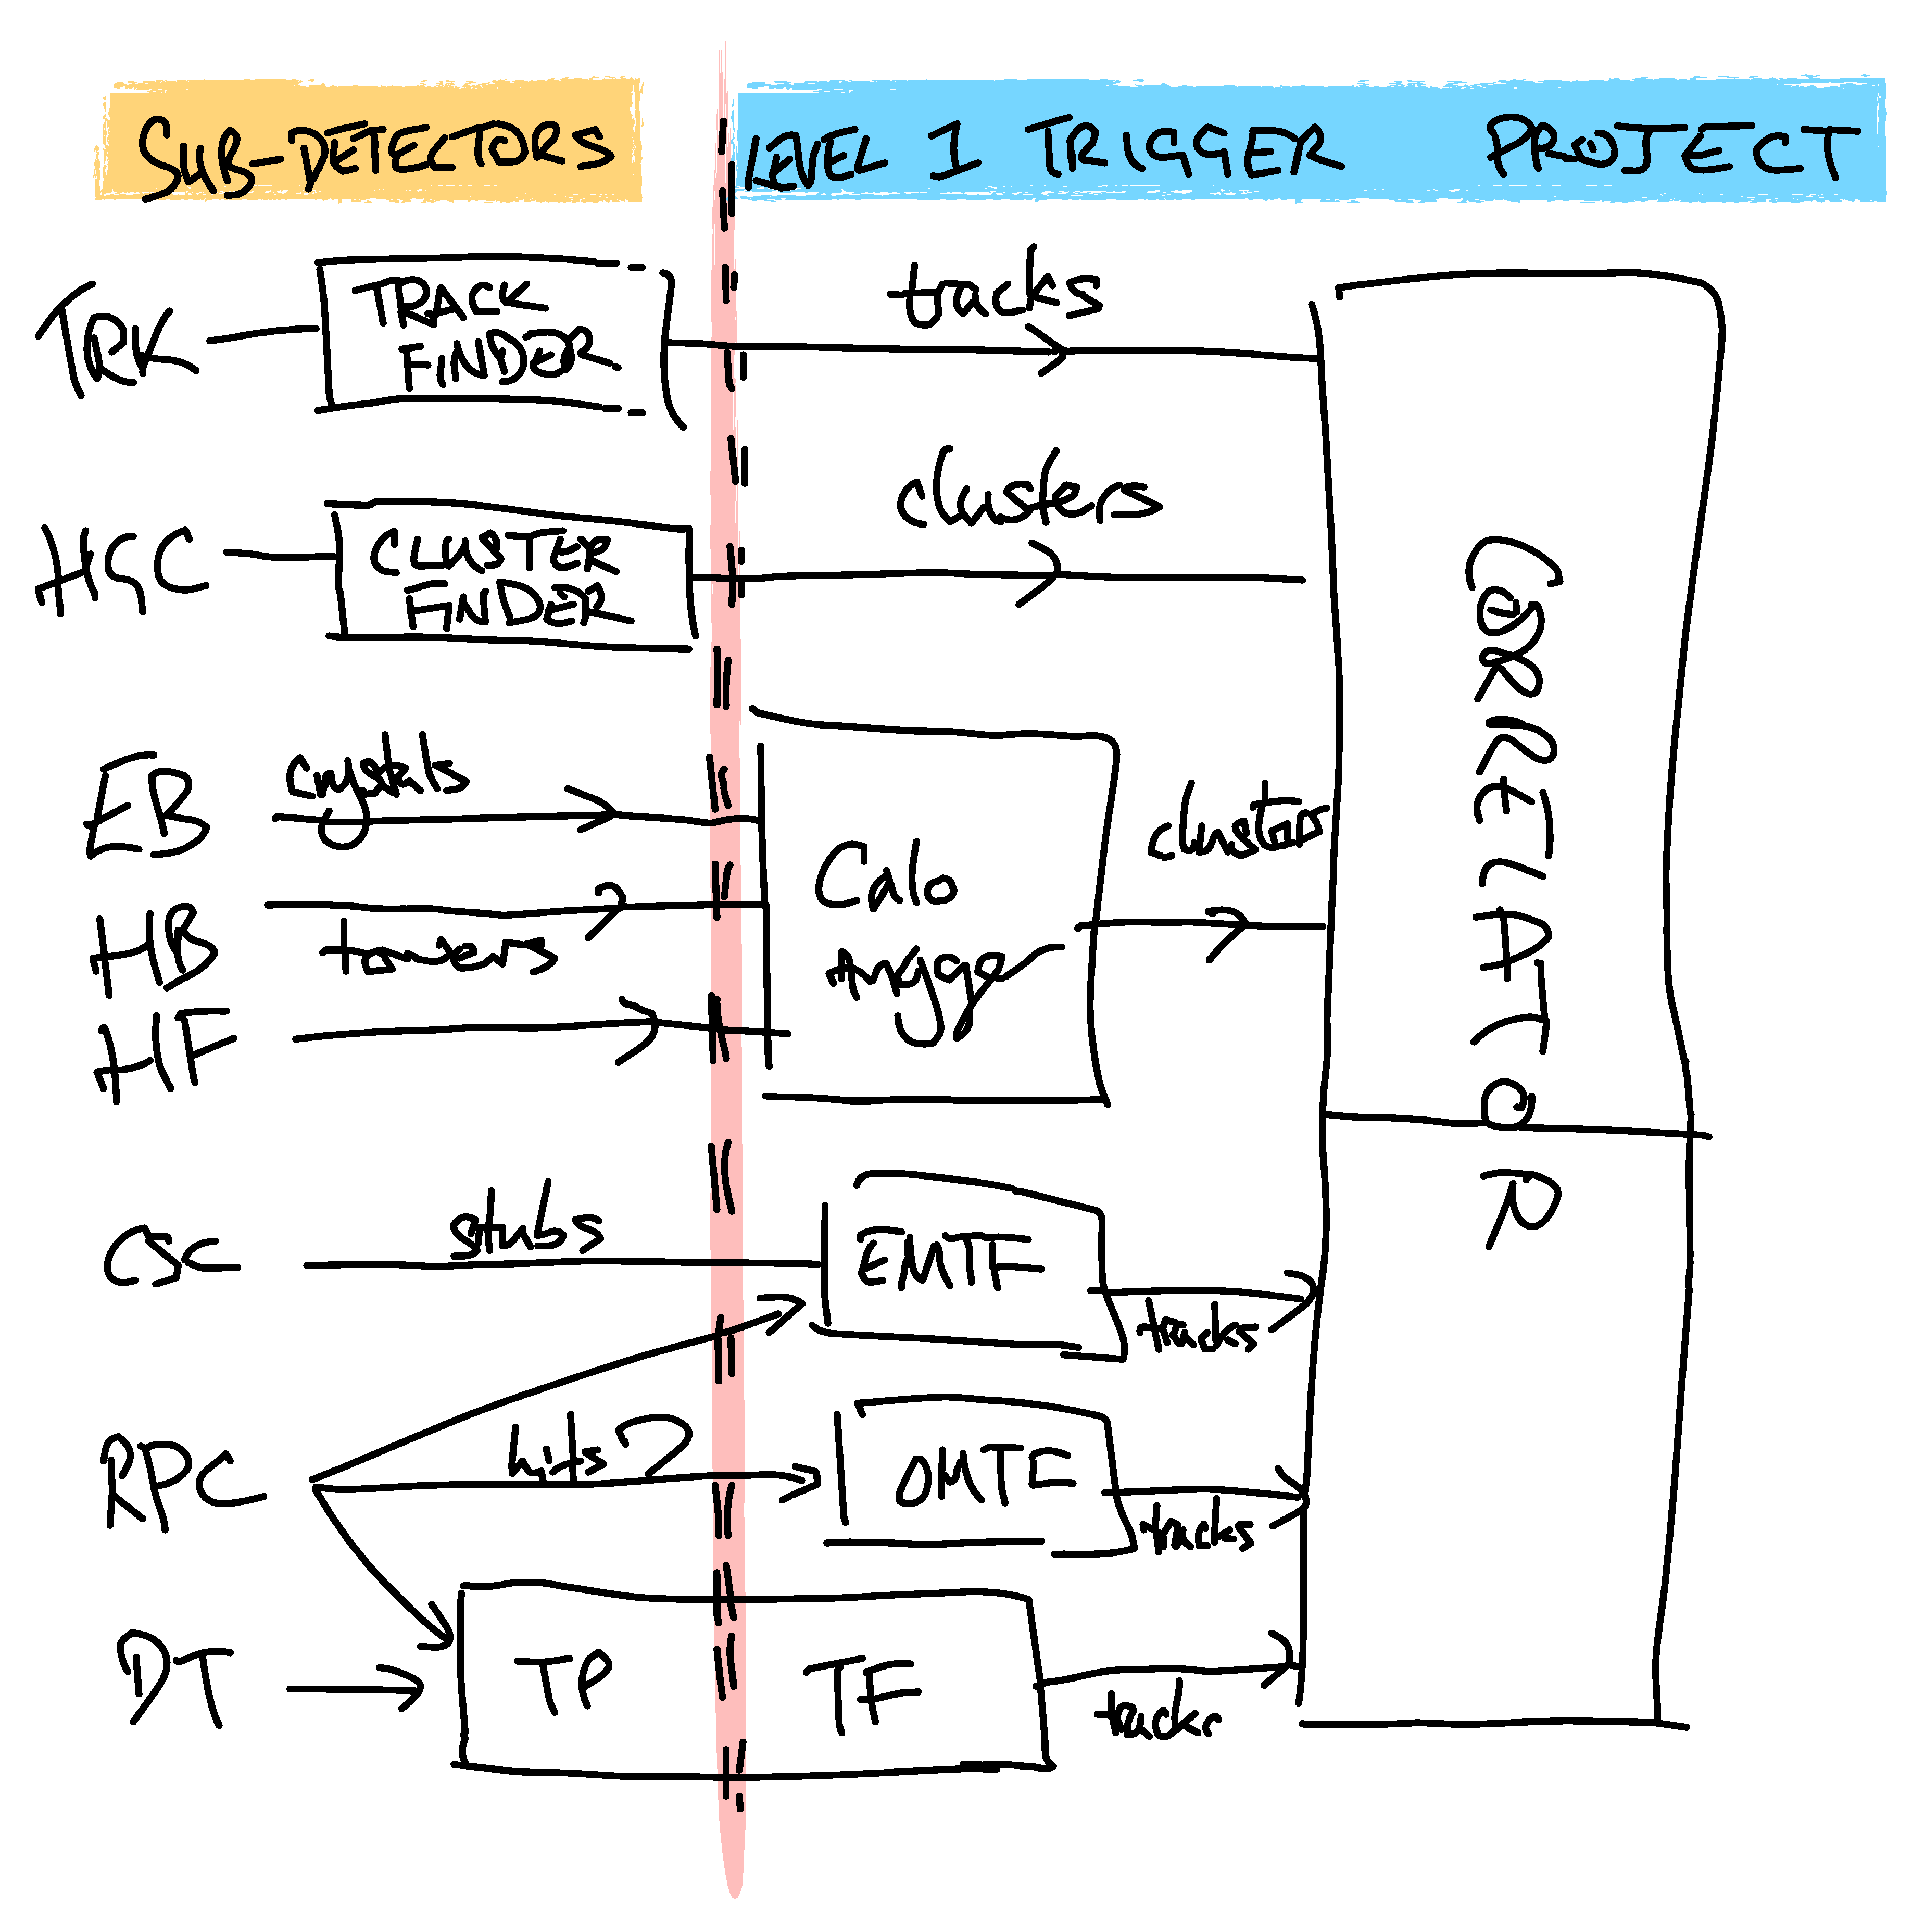
\includegraphics[width=0.6\textwidth] {figures/system.pdf}
\caption{
Overview of the L1 trigger system, courtesy J. Brooke.
\label{fig:overview}
}
\end{figure}

With the addition of the tracking information to the L1 trigger system for the HL-LHC, we can now further expand the capabilities of the system.
Using our experience from offline reconstruction, the particle flow reconstruction algorithm has been successfully demonstrated at CMS.
In this algortihm, detector signals from the tracker, calorimeters and muons are combined and translated into particle candidates such as muons, electrons, charged hadrons, neutral hadrons and photons.
The particle flow algorithm has shown improved physics object resolution and efficiency over more traditional reconstruction techniques. 
In high pileup scenarios, the pileup per particle identification (PUPPI) algorithm, which operates with particle flow candidates as inputs, has been demonstrated to greatly mitigate the physics performance degradation from pileup.  
PUPPI uses vertexing information from the tracks and a QCD-based ansatz to define a weight
of how likely each particle candidates is from pileup.  
The goal of our studies is to implement the principles which make the offline PF and PUPPI algorithms successful 
in the L1 trigger.  

The note is organized as follows.
In Sec.~\ref{sec:algo}, we present the core algorithm in the trigger from hereto on denoted as L1PFP.
In Sec.~\ref{sec:phys}, we then study the physics performance of the algorithm. 
Section~\ref{sec:degradedpf} is devoted to understanding the performance the offline PF and PUPPI algorithms with degraded inputs similar to the trigger.  This is important to benchmark our performance expectations.  
Finally, Sec.~\ref{sec:fw} is devoted to the description of the algorithm and how it is performing in firmware and hardware.  






\clearpage
\section{The core algorithm, L1PFP}
\label{sec:algo}
In the section, we describe the core L1PFP algorithm.

\subsection{Inputs to the algorithm}
\label{sec:algo:input}

\subsubsection{Input format}

The inputs to the L1PFP algorithm are calorimeter clusters, strip tracks and muon tracks. 
The inputs are summarized in Table~\ref{tab:inputs}

\begin{table}[hbtp]
\begin{center}
 \caption{Summary of the inputs to the correlator trigger}
\begin{tabular}{ |c|cc|cc| } 
 \hline
 Subsystem & $N_\text{obj}$ & bits/obj & rate (Kb/BX) & rate (Tb/s)  \\ 
 \hline
 Tracker & 100 & 128 & - & - \\
 Barrel clusters & - & - & - & - \\
 Endcap clusters & - & - & - & - \\
 HF towers & - & - & - & - \\
 muons & - & - & - & - \\
 \hline
\end{tabular}
\label{tab:inputs}
\end{center}
\end{table}

The track inputs are assumed to have a 2\GeV \pt cut on them based on specifications for the track trigger system.

\subsubsection{Calorimeter clustering}

\subsection{The L1PFP algorithm}

Given the inputs defined for the L1PFP algorithm in Sec.~\ref{sec:algo:input}, we now describe
in detail each critical step of the algorithm.
An overview of the algorihm is given in Fig.~\ref{fig:l1pfp}. 
The inputs to the algorithms are in the red boxes: tracks, calorimeter clusters, and muons. 
We classify two types of operations: global and local.  
Global operations require information from the entire detector while local operations require 
only information from one region of the detector. 

\begin{figure}[htb]
\centering
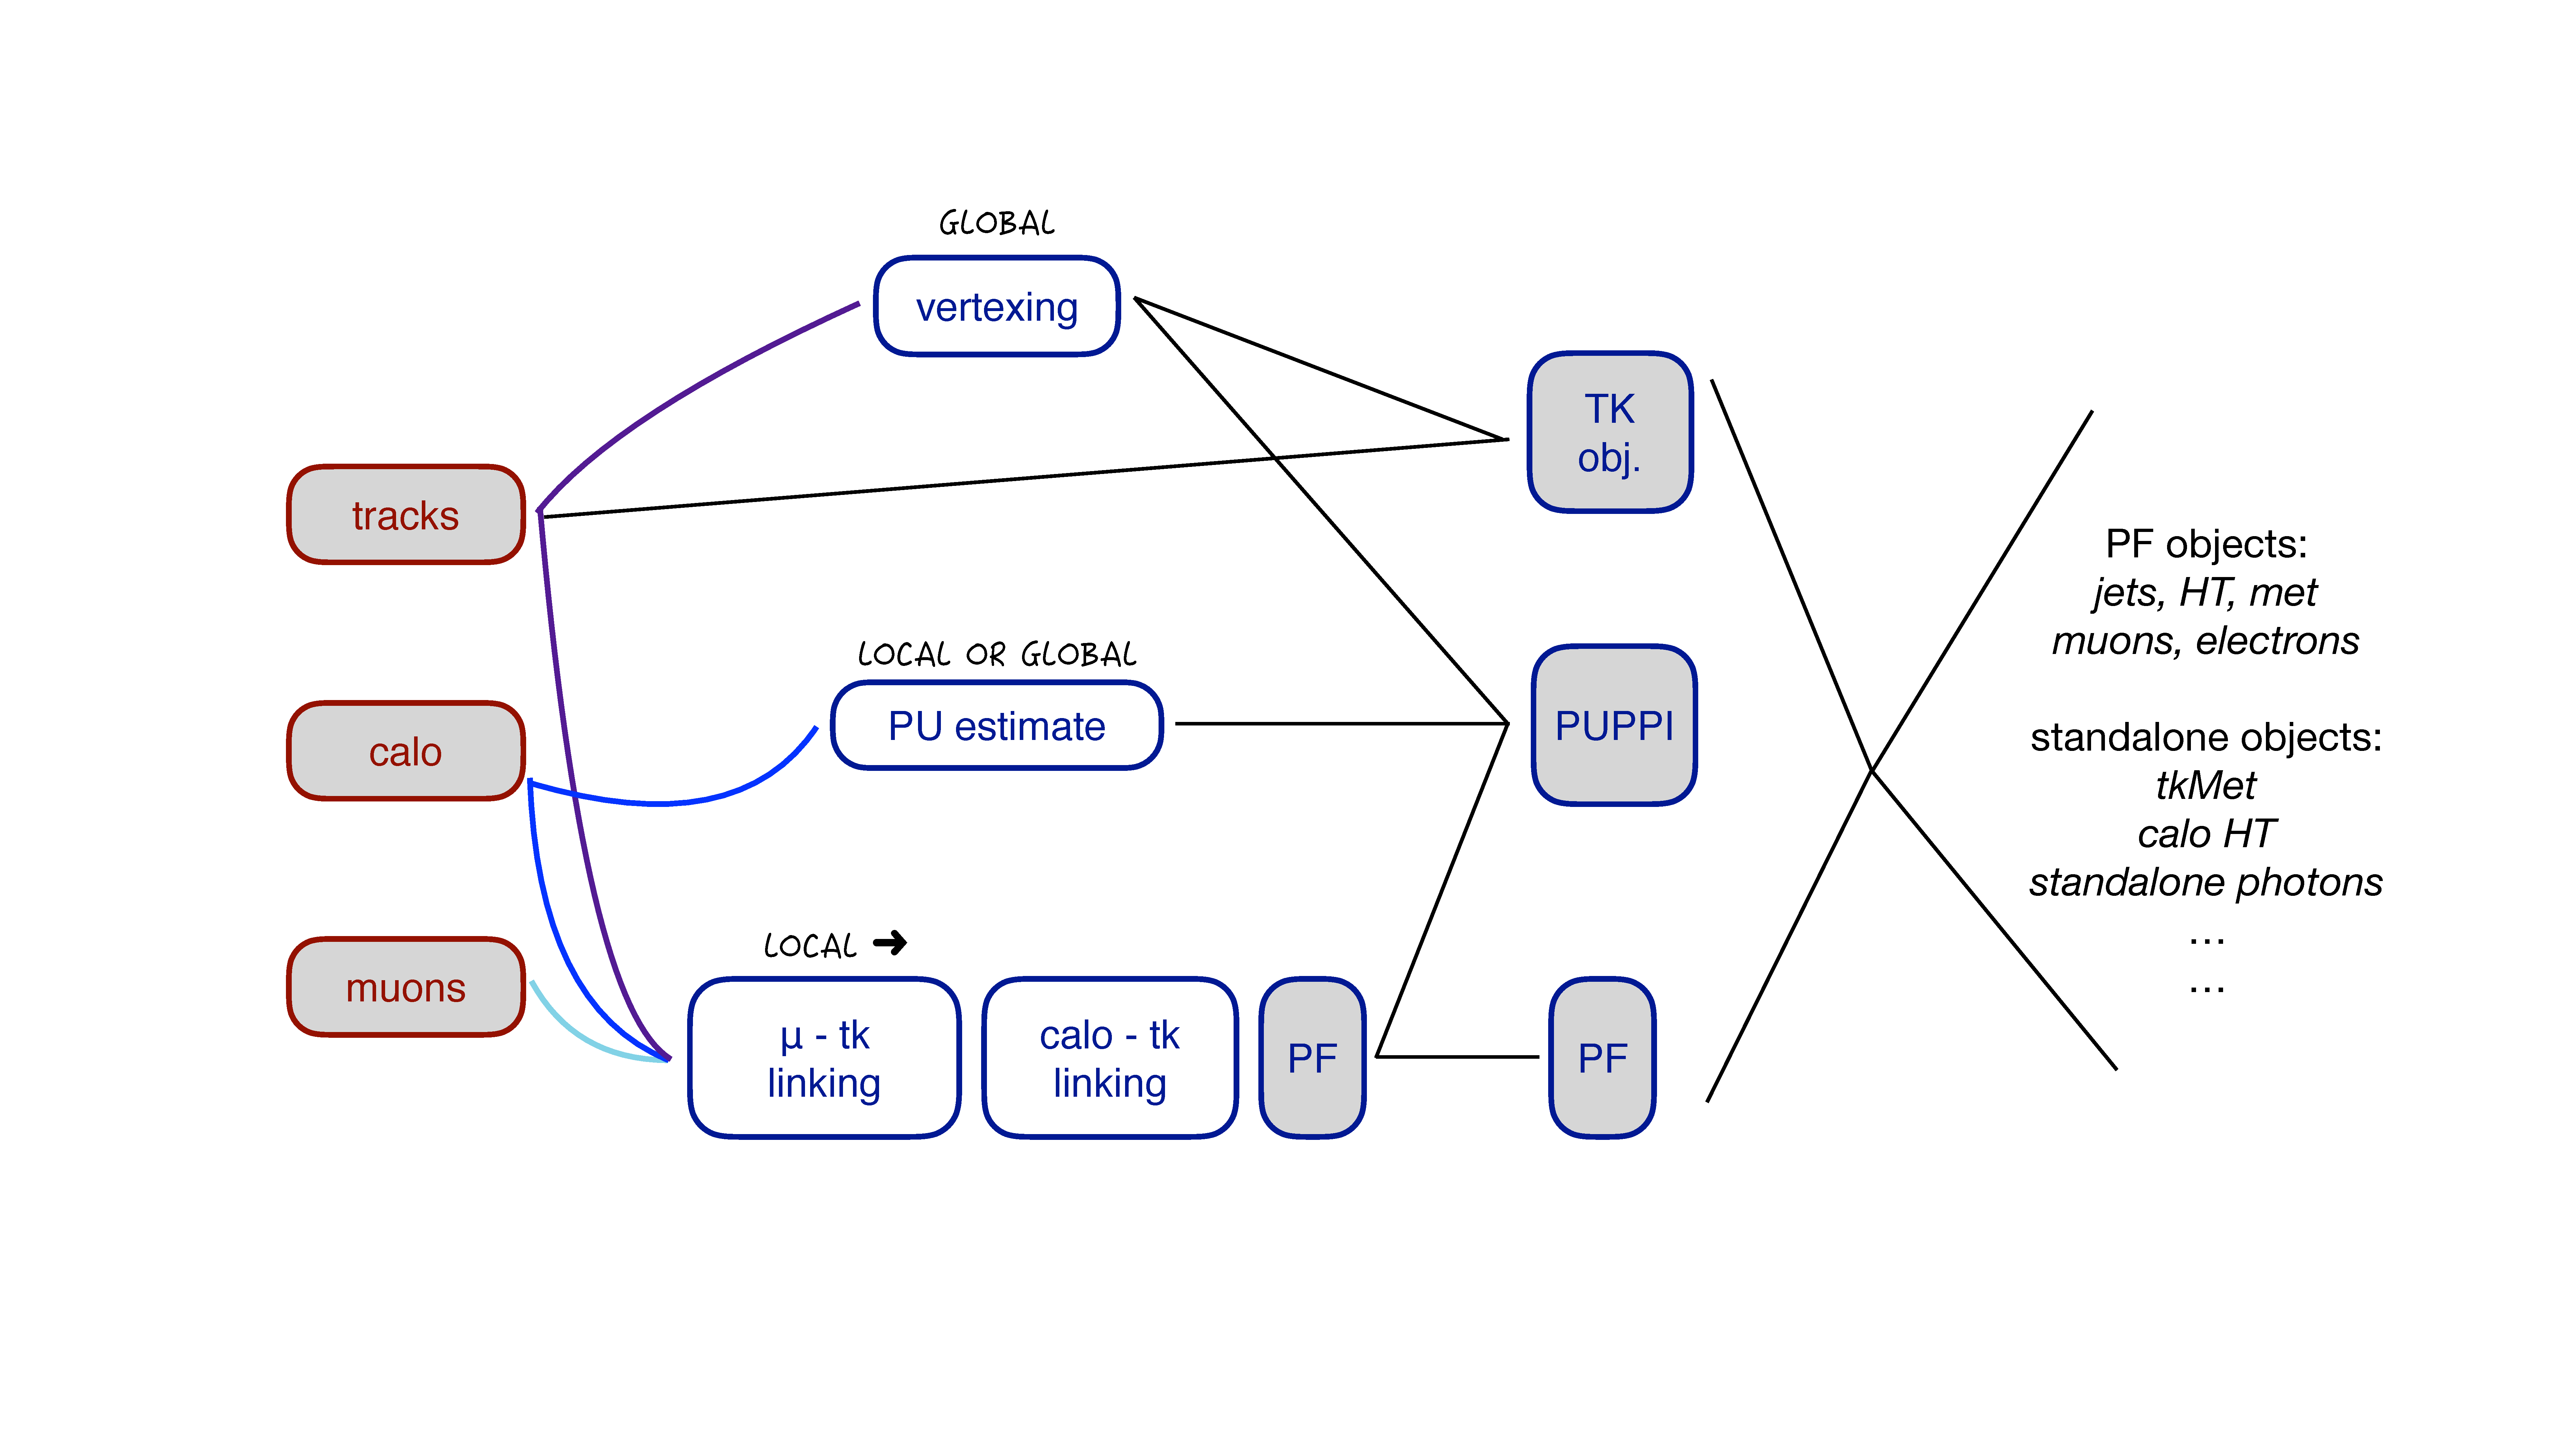
\includegraphics[width=0.9\textwidth] {figures/l1pfp.pdf}
\caption{
Overview of the L1PFP algorithm
\label{fig:l1pfp}
}
\end{figure}

The local operation steps proceed in the following order: 
\begin{enumerate}
\item Track-muon linking: combines muon tracks and tracker tracks to make muon objects
\item Track-calo linking: links calorimeters cells with tracker tracks to define both charged and neutral hadrons and photons and electrons
\item PUPPI: performed in parallel to the vertexing and pileup estimate, estimates the likelihood of being pileup
\end{enumerate}

Each of these, as well as the global operations, are described in further detail below.  
After the computation of the L1PFP particle candidates, the physics objects can be computed such as jets, MET and lepton information.  
It should be noted other standalone objects may also be computed at this stage such as track-based MET and calorimeter based photons.

\subsubsection{Vertexing and pileup estimate}

Vertexing is an extremely important step in the pileup mitigation of any algorithm. 
Pileup interactions occur at different points in the beam spot and differentiating each interaction's z position helps to reject uninteresting pileup interactions. 
We currently follow the histogramming algorithm proposed in~\cite{Contardo:2020886} to do a fast vertexing using the track trigger tracks.
The method bins the tracks in their Z vertex position.  
We bin the tracks from $\delta z = ( -20\cm,20\cm )$ with a bin size of 1.3\mm summing the bin content by track $\pt_{tk}'$ where $\pt_{tk}'$ = $\text{min}(50\GeV, \pt^{tk})$ 
and $\pt^{tk}$ is the track \pt.
We do not allow the track \pt to be greater than 50\GeV in order to minimize the effect from fake tracks.
The primary vertex $\delta z$ is labeled $\delta z_{PV}$ and is defined as the center of the bin with the largest $\Sigma \pt_{tk}'$.
We then define tracks from the primary vertex as tracks within $\delta z_{PV} = \pm 1.95~\mm$

{\color{red} to do: make a few plots to demonstrate vertexing efficiency}



\subsubsection{Track-Muon linking}
\subsubsection{Track-Calo linking}
\subsubsection{Regional definitions}
\subsubsection{Integer emulation}

\clearpage
\section{Physics validation}
\label{sec:phys}
In this section, we compare the physics performance of the algorithm against other possible L1 physics object options.

\subsection{MC samples}

\subsection{Missing Energy}

\subsection{Jets and energy sums}

\subsection{Leptons}

\clearpage
\section{Degraded offline particle flow}
\label{sec:degradedpf}
In this section, we examine the offline particle flow and PUPPI reconstruction algorithms.  
This is very important to understand because it benchmarks the physics performance we find in the previous section. 
We want to study the L1PFP performance with respect to its offline analogs so that we will know
the how close we are to "optimal" performance and what L1 trigger approximations cause the most performance degradation.

\clearpage
\section{Performance in firmware and hardware}
\label{sec:fw}

\clearpage
\section{Summary and outlook}


% >> acknowledgments (for journal papers)
% Please include the latest version from https://twiki.cern.ch/twiki/bin/viewauth/CMS/Internal/PubAcknow.
%\begin{acknowledgments}...ack-text...\end{acknowledgments}
% This will normally be updated with the text available at the time of submission,
% so please add a comment if it has been modified. Such modifications need to be
% approved.
%
\begin{acknowledgments}
\hyphenation{Bundes-ministerium Forschungs-gemeinschaft Forschungs-zentren} We congratulate our colleagues in the CERN accelerator departments for the excellent performance of the LHC and thank the technical and administrative staffs at CERN and at other CMS institutes for their contributions to the success of the CMS effort. In addition, we gratefully acknowledge the computing centers and personnel of the Worldwide LHC Computing Grid for delivering so effectively the computing infrastructure essential to our analyses. Finally, we acknowledge the enduring support for the construction and operation of the LHC and the CMS detector provided by the following funding agencies: the Austrian Federal Ministry of Science, Research and Economy and the Austrian Science Fund; the Belgian Fonds de la Recherche Scientifique, and Fonds voor Wetenschappelijk Onderzoek; the Brazilian Funding Agencies (CNPq, CAPES, FAPERJ, and FAPESP); the Bulgarian Ministry of Education and Science; CERN; the Chinese Academy of Sciences, Ministry of Science and Technology, and National Natural Science Foundation of China; the Colombian Funding Agency (COLCIENCIAS); the Croatian Ministry of Science, Education and Sport, and the Croatian Science Foundation; the Research Promotion Foundation, Cyprus; the Ministry of Education and Research, Estonian Research Council via IUT23-4 and IUT23-6 and European Regional Development Fund, Estonia; the Academy of Finland, Finnish Ministry of Education and Culture, and Helsinki Institute of Physics; the Institut National de Physique Nucl\'eaire et de Physique des Particules~/~CNRS, and Commissariat \`a l'\'Energie Atomique et aux \'Energies Alternatives~/~CEA, France; the Bundesministerium f\"ur Bildung und Forschung, Deutsche Forschungsgemeinschaft, and Helmholtz-Gemeinschaft Deutscher Forschungszentren, Germany; the General Secretariat for Research and Technology, Greece; the National Scientific Research Foundation, and National Innovation Office, Hungary; the Department of Atomic Energy and the Department of Science and Technology, India; the Institute for Studies in Theoretical Physics and Mathematics, Iran; the Science Foundation, Ireland; the Istituto Nazionale di Fisica Nucleare, Italy; the Ministry of Science, ICT and Future Planning, and National Research Foundation (NRF), Republic of Korea; the Lithuanian Academy of Sciences; the Ministry of Education, and University of Malaya (Malaysia); the Mexican Funding Agencies (CINVESTAV, CONACYT, SEP, and UASLP-FAI); the Ministry of Business, Innovation and Employment, New Zealand; the Pakistan Atomic Energy Commission; the Ministry of Science and Higher Education and the National Science Centre, Poland; the Funda\c{c}\~ao para a Ci\^encia e a Tecnologia, Portugal; JINR, Dubna; the Ministry of Education and Science of the Russian Federation, the Federal Agency of Atomic Energy of the Russian Federation, Russian Academy of Sciences, and the Russian Foundation for Basic Research; the Ministry of Education, Science and Technological Development of Serbia; the Secretar\'{\i}a de Estado de Investigaci\'on, Desarrollo e Innovaci\'on and Programa Consolider-Ingenio 2010, Spain; the Swiss Funding Agencies (ETH Board, ETH Zurich, PSI, SNF, UniZH, Canton Zurich, and SER); the Ministry of Science and Technology, Taipei; the Thailand Center of Excellence in Physics, the Institute for the Promotion of Teaching Science and Technology of Thailand, Special Task Force for Activating Research and the National Science and Technology Development Agency of Thailand; the Scientific and Technical Research Council of Turkey, and Turkish Atomic Energy Authority; the National Academy of Sciences of Ukraine, and State Fund for Fundamental Researches, Ukraine; the Science and Technology Facilities Council, UK; the US Department of Energy, and the US National Science Foundation.

Individuals have received support from the Marie-Curie program and the European Research Council and EPLANET (European Union); the Leventis Foundation; the A. P. Sloan Foundation; the Alexander von Humboldt Foundation; the Belgian Federal Science Policy Office; the Fonds pour la Formation \`a la Recherche dans l'Industrie et dans l'Agriculture (FRIA-Belgium); the Agentschap voor Innovatie door Wetenschap en Technologie (IWT-Belgium); the Ministry of Education, Youth and Sports (MEYS) of the Czech Republic; the Council of Science and Industrial Research, India; the HOMING PLUS program of Foundation for Polish Science, cofinanced from European Union, Regional Development Fund; the Compagnia di San Paolo (Torino); the Consorzio per la Fisica (Trieste); MIUR project 20108T4XTM (Italy); the Thalis and Aristeia programs cofinanced by EU-ESF and the Greek NSRF; and the National Priorities Research Program by Qatar National Research Fund.
\end{acknowledgments}
%% **DO NOT REMOVE BIBLIOGRAPHY**
\bibliography{auto_generated}   % will be created by the tdr script.


